
%%% Local Variables:
%%% mode: latex
%%% TeX-master: t
%%% End:

\chapter{实例应用}

\section{案例选取}

为了验证本文联合定权和误差评定的实用性,将本文方法应用到芦山地震以反应其震源机制和误差。芦山地震发生于2013年4月12日,震级超过Mw6级,震源中心在四川省雅安市芦山县附近,是继2008年汶川特大地震以来龙门山断裂带发生的又一强震。地震发生后造成几百人死亡,上万人受伤,受灾人口超过200余万\zhcitep{崔鹏}{cuipeng2013},引起了社会各界关注。在直接造成特大地震灾害的同时,芦山地震还诱发了大量的次生山地灾害,其中主要包括落石、崩塌、堰塞湖、泥石流、滚石和滑坡等\zhcitep{陈晓清}{chenxiaoqing2013}。这些次生灾害造成的人员伤亡和经济损失不低于地震的直接影响,不仅如此,次生灾害还阻塞了紧急救援道路,拖慢了救援的进度。地震诱发的大量崩塌、滑坡又为泥石流活动提供了丰富的物质源料,促进了泥石流灾害活跃,并致使在后期暴雨作用下产生了更为严重的泥石流灾害。

选取该地震有以下方面考虑:首先,芦山地震MW震级在6-7级之间,既可以保证足够的远场地震波能量,同时又可避免过大震级的震源复杂性对波场影响;其次该地震发生后,引起了大量学者的关注,对其震源机制作了大量研究,结果可用于参考对比。

利用远场台站体波(P,S)数据进行震源机制反演。需要注意的是我们仅使用了远场体波数据,一方面是因为近场波形反演对震源区局部的浅层结构误差敏感,根据\zhcitet{郑勇}{zhenyong2013}和\zhcitet{高原}{gaoyuan2013} 芦山地震恰巧位于地壳厚度和波速结构横向变化剧烈之处。\zhcitet{谢祖军}{xiezujun2013}的研究表明不同一维模型对近震反演的震源参数影响高达到10°,而远场波形则对地壳及上地幔的横向非均匀性和震源破裂细节的复杂性不敏感;另一方面,在前文中提到体波相位的系统性误差理论上可通过平移因子K来抵消,但面波具有频散效应,使得K无法补偿结构误差对其相位的影响,且面波易受浅层结构横向非均匀性影响,所以反演时舍弃了面波数据。

\section{数据处理}

选取IRIS提供的54个震中距在30°-90°之间且方位分布较均匀的台站(如\reffig{fig4_01}所示)宽频带P及SH波数据,以AK135模型\citep{Kennett1995}作为地球参考模型进行反演。经过多次数据挑选进行除错,最终选取了质量较高的102道相对P波到时(-10s,30s)的时窗并进行(0.01-0.1Hz)带通滤波(基于频谱分析及滤波试验)的P波数据。SH波数据总共挑选了38道,带通滤波频率为(0.005-0.06Hz),时窗选为相对其到时(-30s,100s)。格点搜索时震源机制(走向、倾角、滑动角)的搜索步长为1°,震源深度的步长为1km。为了检验本文提出的w1*w2联合权重的优化效果,用Fit拟合函数分别尝试了w1*w2加权和仅用w1或w2加权三种方案的反演以进行比较。
\begin{figure}
\centering
  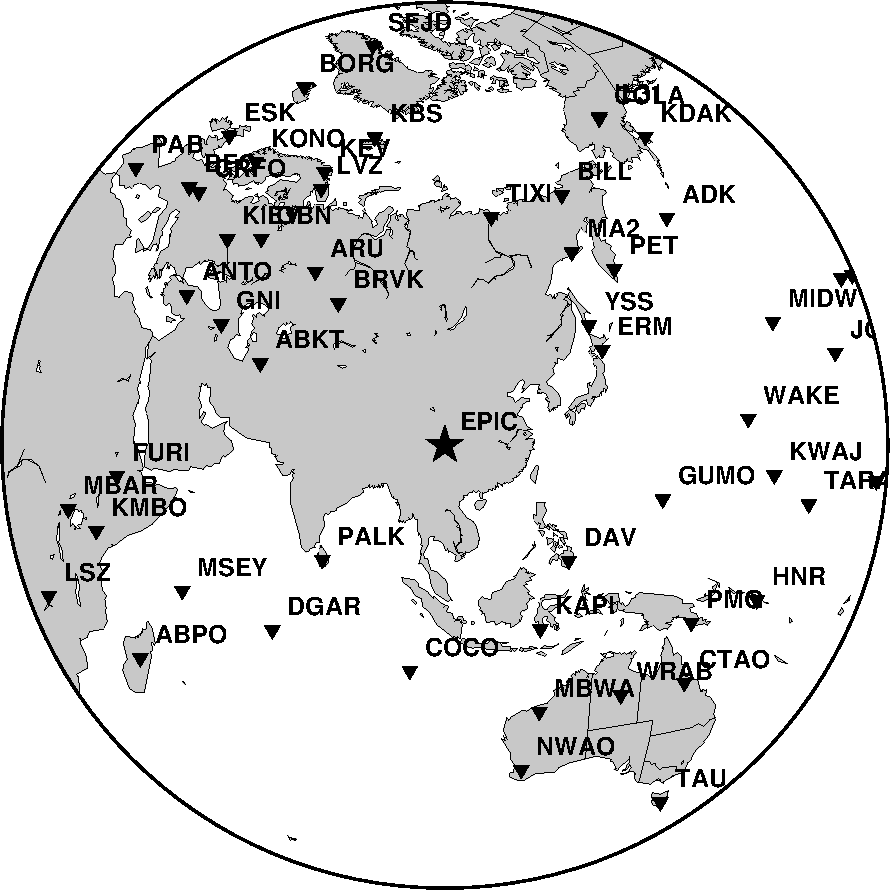
\includegraphics[scale=0.8,angle=0]{fig4_01.pdf}
  \caption{波形反演所用数据的台站分布,其中五角星表示震中,倒三角表示台站}
  \label{fig4_01}
\end{figure}

\section{结果分析}

本文三次反演的结果如\reftab{tab401}所示,w2加权与w1*w2加权的反演结果非常接近,而与w1加权结果差别稍大。总的来说三次反演结果均较一致,说明该数据分布较理想,加权是为了使反演结果更合理的一种微调。以下详细分析三次反演的差异以体现不同加权的优劣。
\begin{table}[ht]
\centering
\caption{三种加权方案反演芦山地震的结果}
\label{tab401}
    \begin{tabular}{c c c c c c c}
    \hline
    加权方案 & 深度/km  & 走向/$\degree$ & 倾角/$\degree$ & 滑动角/$\degree$ & 震级($M_w$) & 拟合度(Fit) \\
    \hline
    W1		& 16  & 202 & 47 & 96 & 6.49 & 0.7827 \\
    W2		& 18  & 213 & 41 & 95 & 6.41 & 0.5822 \\
    WT		& 17  & 211 & 41 & 94 & 6.41 & 0.6052 \\
    \hline
    \end{tabular}
\end{table}

首先分析三次反演的拟合度大小以体现w1的作用,从反演理论可知适当增加高质量数据的权重可以减小反演结果的误差,并使理论数据与观测值吻合得更好。从\reffig{fig4_02}可以发现w1*w2反演与w2单独加权反演的拟合度曲线非常接近,不过后者的拟合度始终略高于前者,这是因为w1*w2加权反演对数据信噪比进行了分析,使得质量较差的数据在反演中的权重有所下降,减弱了较大随机噪声的干扰,导致数据拟合度有所提升。另一方面,w1单独加权的反演拟合度是三次反演中最高的,这也正是由于w1加权是基于数据随机噪声情况调节权重,使反演的拟合度尽量最高。三次反演的拟合度大小情况恰好符合w1的理论预期效果。
\begin{figure}
\centering
  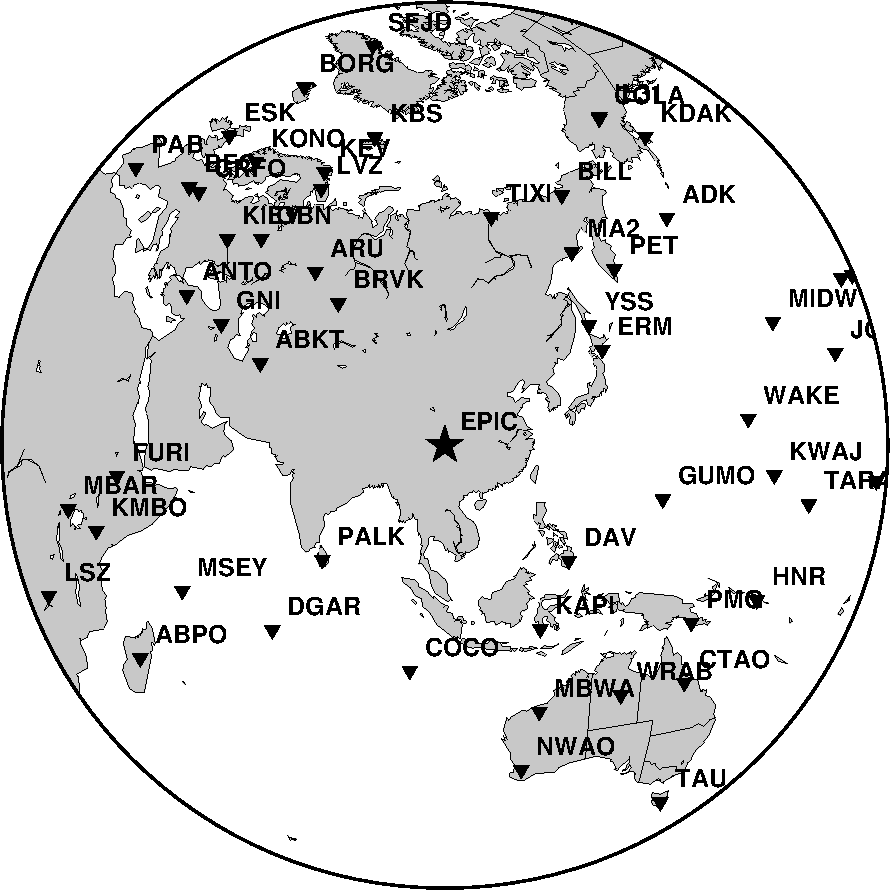
\includegraphics[scale=0.4,angle=0]{fig4_02.pdf}
  \caption{三种反演方案拟合度随震源深度的变化曲线}
  \label{fig4_02}
\end{figure}

但是使拟合度最高的单独w1加权反演却不见得是三次反演中最好的,以下从震源深度和震源机制的约束效果方面讨论w2的效果。从如\reffig{fig4_02}所示的震源深度格点搜索过程中,可以发现三次反演的全局最值均在18km附近。其中w1*w2反演与w2反演均只有这一个极值,而w1加权反演则在33km附近还出现了另一局部极值,这说明在同样的数据分布和反演方法情况下,w1加权反演对该地震的震源深度约束较差。这是因为pP及sP震相在远震震相中对深度约束作用最好,在本文低频滤波情况下,pP及sP深度震相与P震相融合在一起,包含在P波时窗中,故P波信息对震源深度约束较好。而对于剪切位错源,S波振幅通常比P波振幅大很多,未经w2振幅调节会导致P波的信息在反演中得不到充分体现,反演结果更多地关注S波的拟合,所以三次反演中单独w1加权反演对震源深度约束效果略差于另两次反演。

另一方面,从\reffig{fig4_03}可以看到w1单独加权与w1*w2加权反演过程中,不同深度对应的最佳震源机制情况。很明显w1*w2联合加权的深度搜索过程中震源机制一直较为稳定,而w1单独加权反演中不同深度对应的震源机制差异较大,甚至在全局最值附近走向的变化也较为明显,这表明w1*w2反演的震源机制稳定性比w1单独加权反演要好。这是因为w2权重更好地平衡了不同振幅波形在反演中的影响,使得各种震相信息在反演中得到合理的充分利用,从而能更好地约束震源机制解。
\begin{figure}
\centering
  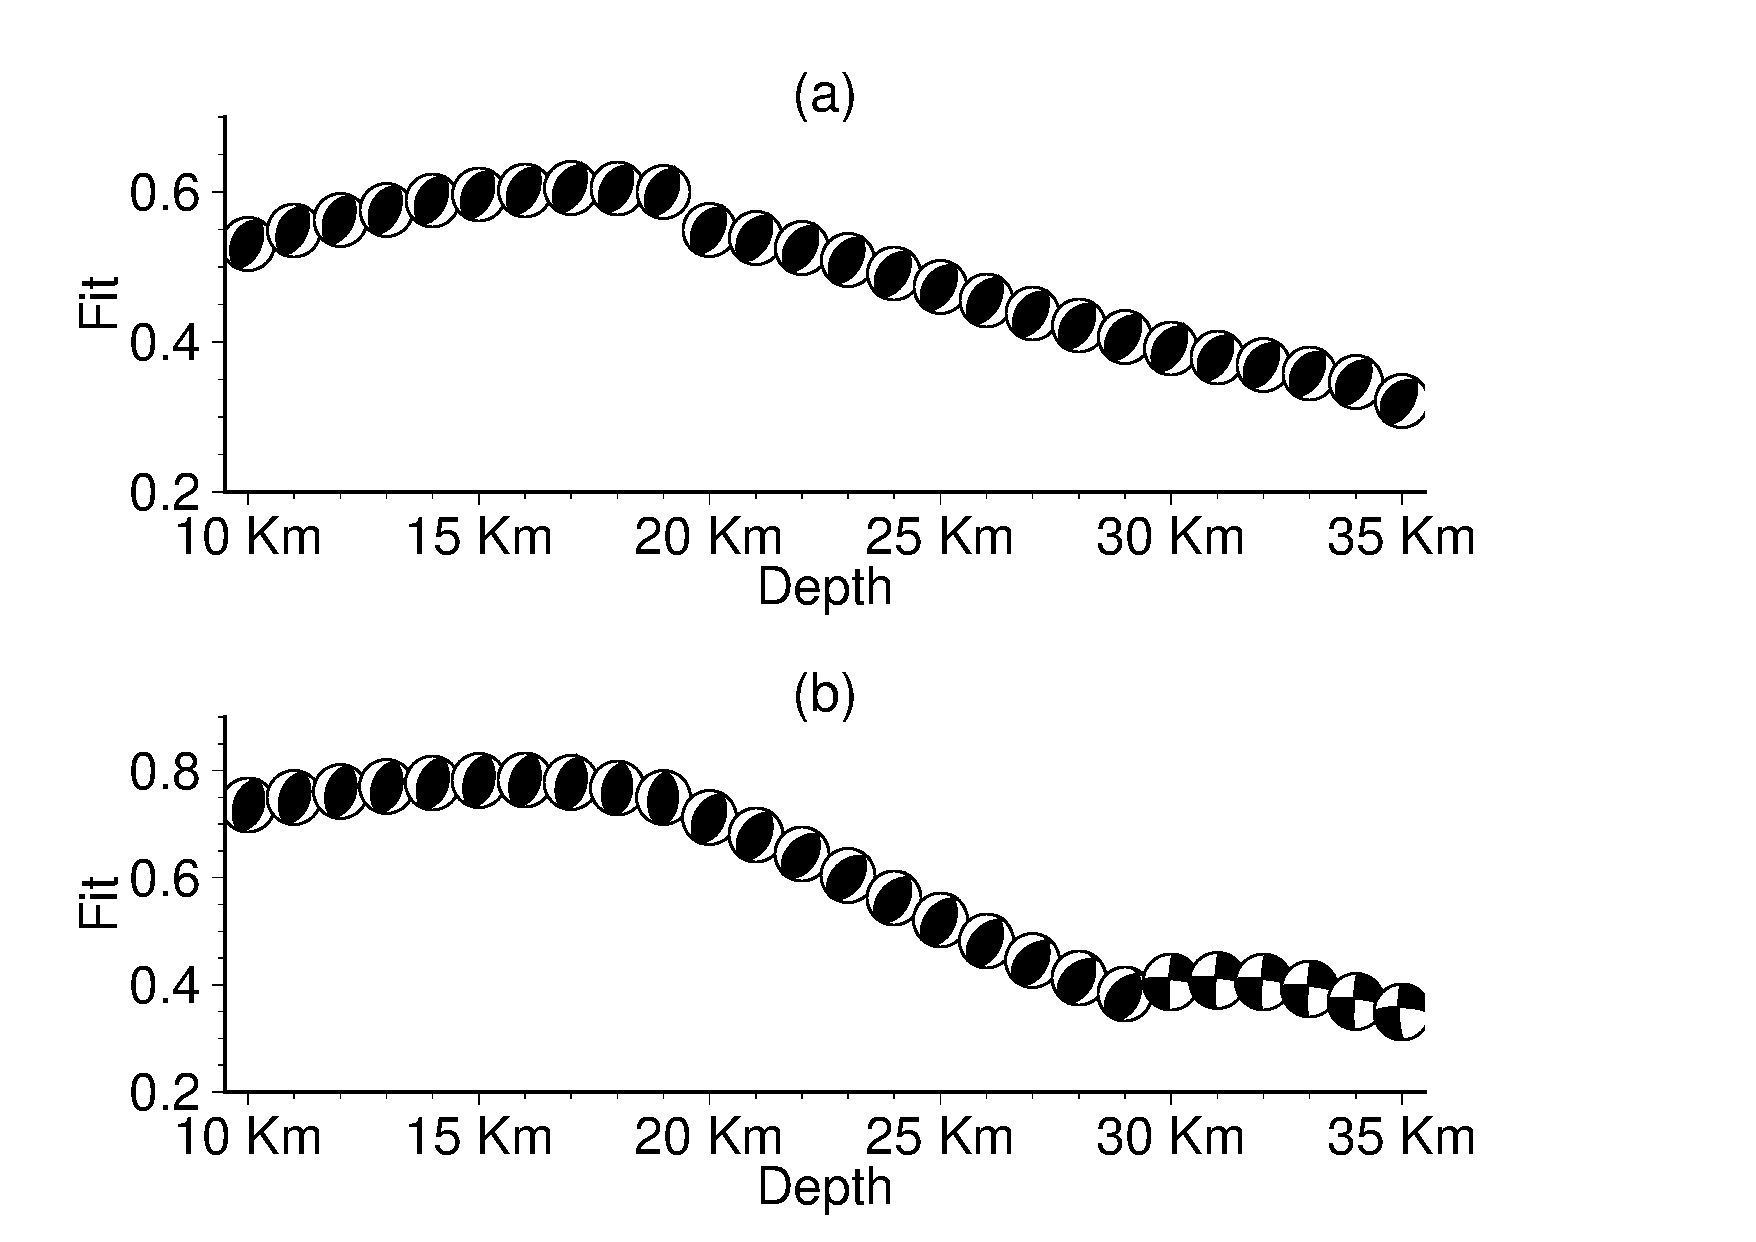
\includegraphics[scale=0.4]{fig4_03.pdf}
  \caption{ (a)(b)分别为wt(w1*w2)加权w1加权反演各震源深度对应最佳解}
  \label{fig4_03}
\end{figure}

综上分析,w1权重能有效减弱随机噪声影响,w2权重能使反演合理充分利用各种震相信息,更好约束反演结果,所以w1*w2联合加权的结果应该是三种加权反演结果中最优的。本文w1*w2加权反演的所有台站理论与观测波形拟合情况如\reffig{fig4_04}所示。可以看到P波及SH波拟合得都不错,相位及其振幅均匹配得非常好。值得注意的是,同一台站的P波Z与R分量的时间平移参数非常一致,这是因为平移因子是由地震定位,发震时刻及地球速度结构等系统性误差引起的,且理论上其误差影响对于同一台站的同一震相应是相同的。此外,对于不同震中距台站的波形,拟合情况均相当,表明反演综合考虑了所有波形的信息。
\begin{figure}
\centering
  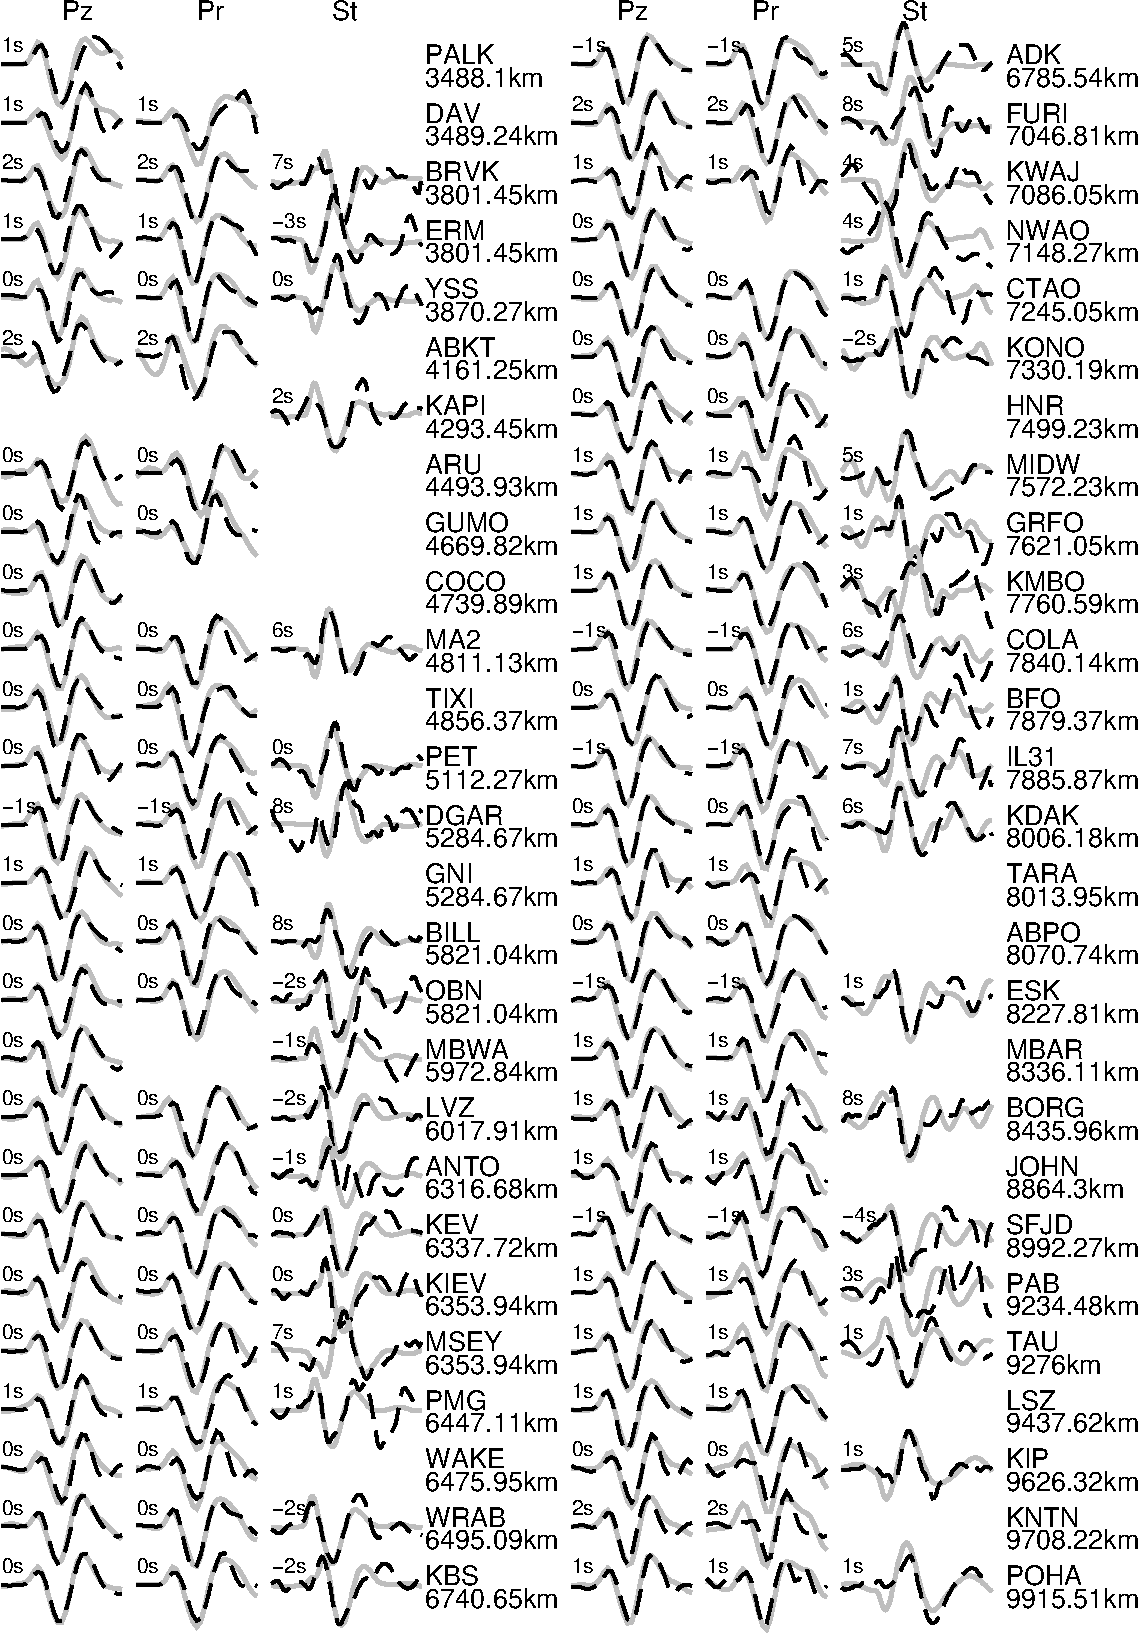
\includegraphics[scale=0.78]{fig4_04.pdf}
  \caption{ wt加权反演波形对比图,虚线为观测波形,实线为理论波形,波形右侧分别为台站名、震中距(km)。各道波形的左上方为到时差,正值表示理论到时相比实测波提前,负值相反}
  \label{fig4_04}
\end{figure}

\section{讨论和结论}

芦山地震后,各研究者分别对该地震震源机制进行了详细研究。\zhcitet{曾祥方}{zengxiangfang2013}利用\citet{Hardebeck2002}改进的P波初动极性反演方法及近远震波形反演方法得到了较一致的震源机制解,且利用误差曲线分析了倾角和深度的可靠性;\zhcitet{刘杰}{liujie2013}、\zhcitet{吕坚}{lujian2013}利用CAP方法对近震波形反演得到了芦山地震震源机制解,其中吕坚在波形反演基础上利用余震分布进一步约束了发震断层面;\zhcitet{谢祖军}{xiezujun2013}利用CAP方法分别对近震、远震及近远震联合反演进行对比以得到最佳震源机制。相关研究所得的结果均列于表2中,各结果的分布基本为震源深度范围(12-22km),震源机制(走向200-220°,倾角33-50°,滑动角90-110°),Mw震级(6.4-6.7)。本文结果基本在此分布范围内,仅Mw震级略小,这一方面可能是由于本文的Fit函数为了降低了系统性误差对震源机制的影响,将振幅误差归并到震级评估中;另一方面因为各学者所用的数据及参考模型不尽相同,且除了速度结构、地震定位以及发震时刻的不精确,理论波形的计算方法也可能导致系统性误差,不同程序算得的理论波形虽然相位一致,但振幅也会有一定差异\citep{Herrmann1985}。此外,\zhcitet{高原}{gaoyuan2013}对地震重定位得到主震震源深度17.8km,\zhcitet{房立华}{fanglihua2013}用三维速度模型进行双差重定位给出的震源深度为17.2km和17.6km,重定位结果均与本文给出的17km震源深度非常接近,其中房立华使用了接近震中附近的三维速度模型,并用流动观测台站对早期发生的地震进行校正,结果是较为可信的。

芦山地震震源位于龙门山断裂带,在该区域由于同时受到西北部青藏块体向东的挤压作用,以及东南部四川盆地坚硬地壳的阻挡,使得青藏块体东缘下方的地壳物质东流,进而导致软弱的下地壳物质向上逆冲挤出,最终形成逆冲型的东南走向的龙门山断裂带\citep{Zhang2013}。该断裂带主要由4条大断裂构成\zhcitep{邓起东}{dengqidong1994},其整体走向为SW向\zhcitep{李智武}{lizhiwu2008}。可是从整体来看,该断裂带南北段走向具有明显的差异性\citep{Jia2006,Arne1997},\zhcitet{郭正吾}{guozhengwu1996}和\zhcitet{邓康龄}{dengkangling2007}均发现芦山地震震源区所处的南段走向相较于北段而言,有更南偏倾向。龙门山断裂带南段因受喜马拉雅期印-亚碰撞事件的重大影响,显示与松潘-甘孜褶皱带有密切关系,推断其为晚白垩世古近纪沉降中心,南段的断裂活动性延续时间较晚,直到喜马拉雅期基本定型,但现今仍在发育\zhcitep{李智武}{lizhiwu2008}。

龙门山断裂带区域的构造及地下结构一直是大家研究的热点,\citet{Zhang2013},\citet{Wang2010},\zhcitet{张忠杰}{zhangzhongjie2009}和\citet{Zhang2011}等研究者的研究成果表明,龙门山地区的地壳速度结构处于横向变化剧烈处,存在明显的不均匀性。根据\zhcitet{雷建设}{leijianshe2009}对龙门山断裂带地壳结构的研究,芦山地震的震源恰巧在P 波速度变化较大的区域。芦山地震震中与龙门山断裂带南段断层分布(断层数据来自\zhcitet{邓起东}{dengqidong2002})如\reffig{fig4_05}所示,由图可知震中位于南段前山断裂和山前隐伏断裂之间,地质调查结果\zhcitep{徐锡伟}{xuxiwei2013}显示芦山地震的发震断层为一条现今尚未出露地表、其上断点仍埋藏在地下地壳中的一条盲逆断层,无法直接从地表露头来观测震源断裂处走向情况,但是本文反演得到的震源机制显示的走向211°与震源区域断层整体走向基本吻合,表明反演得到的走向具有合理性。\zhcitet{唐荣昌}{tangchangrong1991},\zhcitet{李勇}{liyong2006},\citet{Densmore2007},\zhcitet{陈国光}{chenguoguang2007}等人的研究表明龙门山断裂带总体运行表现为为由北西向南东的逆冲 ,并且同时兼具有右旋走滑的特性, 整条断裂带的冲断运动由北西向南东扩展,但由于受到后山、中央、前山三条断裂带的阻碍作用,断裂带的北段和中段的山前断裂并没有明显地显现出逆冲的特征,可是芦山地震所处的南段区域却不同,其山前断裂带明显受到了冲断运动的影响,发生了较为强烈的冲断和摺皱变形,为震源所处的盲逆断层孕震提供了有利条件,与本文反演得到的滑动角所代表的逆冲型断裂发震的运动背景一致。
\begin{figure}
\centering
  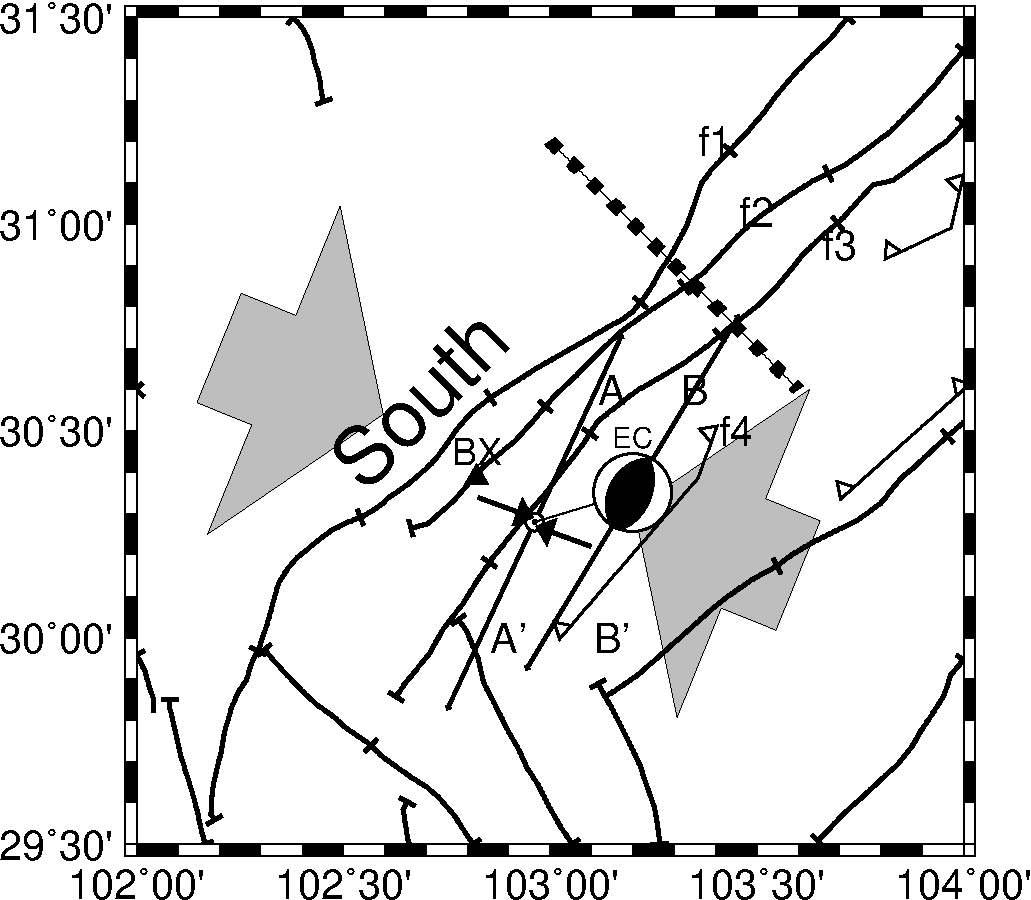
\includegraphics[scale=0.6]{fig4_05.pdf}
  \caption{ 震源区域断层与应力分布, f1,f2,f3,f4为龙门山断裂带的主要四大断裂,灰色大箭头为区域平均应力,黑色小箭头为本文震源机制对应的主压应力}
  \label{fig4_05}
\end{figure}

由于芦山地震发震断裂为盲断裂,难以直接观测发震断裂的空间构造,通过余震分布可以一定程度重现发震断裂的结构信息,\citet{zhangguangwei2013}通过双差定位发现在空间分布上主震西南方向余震分布较广、且较为集中,余震主要向西南方向扩展(\reffig{fig4_05}中AA'剖面),其剖面方向与本文震源机制的走向线BB'近乎平行,说明余震基本沿主震断层面破裂分布。

断层构造活动通常与该区域的应力分布有着密切关系,\zhcitet{孟文}{mengwen2013}实地钻孔测量研究结果表明龙门山断裂带的水平应力占主导作用,且南段的优势方向为NWW向。根据青藏高原内部存在下地壳通道流的观点\citep{Royden1997,Clark2000,Meng2005,Burchfiel1995,Harris2007},松潘-甘孜地体极有可能俯冲到四川盆地之下\zhcitep{楼海}{louhai2010},从而使得龙门山断裂带南段与青藏高原东部具有较好的连接性,是青藏高原东缘的活动边界,因此龙门山断裂带南段最大主压应力方向与区域应力场方向一致,为NW-NWW向,孟文等的钻井数据显示距震中较近的宝兴钻井点主应力方向为N80°W至N74°W,另一钻井结果表明宝兴主应力方向为N60°W\zhcitep{秦向辉}{qinxianghui2013},上述区域应力方向以及实际钻井没得的主应力方向均与本文反演所得的震源机制主应力方向一致。

研究表明, 快剪切波偏振的优势方向一般与原地主压应力方向一致\citep{Gao2011,Gao2012},\zhcitet{高原}{gaoyuan2013}用剪切波分裂的方法计算发现位于芦山地震震中东北方向的龙门山断裂带中南段的台站快剪切波偏振的优势方向近似为NW 向,与断裂带走向近似垂直;而在芦山地震震中西南方向的龙门山断裂带南段靠近鲜水河断裂处,快剪切波偏振方向表现得比较离散,但平均方向为近EW方向,所以地理位置位于其中间的震中区的偏振优势方向极有可能在NW与EW之间。此外\zhcitet{赵博}{zhaobo2013}利用力轴张量法计算得到的芦山地震余震分布区的平均压应力方向约为112°,如\reffig{fig4_05}中灰色大箭头所示。本文震源机制(走向211°,倾角41°,滑动角94°)对应的P轴近水平,与各向异性分析及力轴张量计算法得到的应力结果有很好的一致性。上述钻井实测资料,应力计算资料结果相互吻合,均与本文震源机制表现出一致性,表明芦山地震主要为区域NWW向水平应力长年积累的一次应力释放。
